\section{Experiments}
\noindent{\textbf{Data}} To fairly evaluate the effect of cycle regularization, we use the datasets released by AtlasNet and Pixel2Mesh respectively. Their model sets are both subsets of ShapeNet \cite{shapenetdata} and they both used the rendered image from \cite{3DR2N2}. The absolute size and position of the models and the sampled points as ground truth are not processed in the same way in these two datasets, which makes it unreasonable to compare them all together. However, this does not prevent us to show the effect of our regularization technique separately.

\noindent{\textbf{Training}}
Unless specifically explained, the network models shown in this paper are trained as follows: The parameters for image encoders and forward 3D decoders $\theta_f$ are initialized with parameters released by AtlasNet \cite{atlasnet} and Pixel2Mesh \cite{pixel2mesh} respectively. The parameters for inverse decoders $\theta_g$ are randomly initialized. We use the ADAM \cite{adam} optimizer with the same learning rate as in the original codes of AtlasNet and Pixel2Mesh respectively. We use $\lambda=0.25$ as an empirical choice for the weight of our cycle regularization term. Up till this submission we haven't explored more training strategies for better numerical results yet.

\noindent{\textbf{Evaluation criteria}}
In order to quantitatively evaluate the issue of self-intersection and self-overlap, we count the percentage of self-intersected triangles (``SI") over the total number of triangles. For this evaluation, we provide our code in the supplemental material which can calculate the ``SI" for a input mesh.  
We also use the value of Chamfer distance (``CD") as the original AtlasNet and Pixel2Mesh to evaluate how well the generated mesh approximate the target shape. For the evaluation of Chamfer distance we used the codes that are already implemented by AtlasNet \cite{atlasnet} and Pixel2Mesh \cite{pixel2mesh}.

\noindent{\textbf{Mesh generation and visualization}} Since we are addressing a issue regarding the quality of generated mesh, any post-processing used in AtlasNet \cite{atlasnet} is not used in our experiment. All the triangulations are directly transfered from the predefined surface. We do not divide the triangles to get denser vertex either. The meshes from AtlasNet all have 2500 vertices and about 4k faces. The meshes from Pixel2Mesh all have 2466 vertices and 4928 faces.

To better expose the issue we are addressing in this paper, we render the generated mesh in the software MeshLab and use the ``gooch.gdp" in the software as our shader. In such mode the triangles are rendered golden at front and bluish at back. The golden region and bluish region interlacing at surface evidently indicates the self-intersected surfaces.

\begin{table*}
	\caption{Test error on AtlasNet trained with(\textbf{ours}) and without cycle regularization. Chamfer distance(CD) ($10^3$ times) and percentage of self-intersected(SI) faces are reported. ``AE" stands for the shape auto-encoding task, and ``SVR" stands for single view reconstruction task. Sphere means that the models are using sphere as predefined surface to sample points from. The mean is data-wise as it is implemented in the evaluation code of AtlasNet}
	\label{tab:atlas}
	\centering
	\begin{tabular}{c|rc|rc|rc|rc|}
		\diagbox{Category}{CD,SI}{Model} &\multicolumn{4}{c|}{AE-sphere}&\multicolumn{4}{c|}{SVR-sphere}\\
		\cline{2-9}
		~& \multicolumn{2}{c|}{without-cycle} & \multicolumn{2}{c|}{ours} & \multicolumn{2}{c|}{without-cycle} & \multicolumn{2}{c|}{ours} \\
		\hline
		cellphone&1.3,&0.53\%&1.4,&3.4e-3\%&3.8,&1.4\%&3.7,&2.7e-4\%\\
		watercraft&1.5,&2.3\%&1.8,&6.8e-4\%&4.3,&7.4\%&4.3,&2.6e-4\%\\
		monitor&1.8,&1.8\%&2.0,&9.8e-4\%&6.9,&3.4\%&6.5,&9.8e-4\%\\
		car&1.8,&0.52\%&1.8,&8.0e-4\%&3.9,&0.47\%&3.8,&1.8e-3\%\\
		couch&1.9,&2.5\%&1.9,&8.8e-4\%&5.1,&2.0\%&4.9,&1.7e-3\%\\
		cabinet&2.0&2.3\%&2.2,&1.2e-2\%&5.3,&3.6\%&5.2,&4.3e-3\%\\
		lamp&2.7,&14\%&3.4,&5.5e-2\%&13.2,&19\%&13.1,&2.0e-2\%\\
		plane&1.0,&18\%&1.2,&1.9e-3\%&2.6,&18\%&2.6,&2.9e-3\%\\
		speaker&2.9,&0.77\%&2.9,&1.1e-3\%&10.2,&1.7\%&9.6,&3.1e-4\%\\
		bench&1.3,&11\%&1.6,&7.4e-3\%&4.0,&12.3\%&3.9,&1.6e-2\%\\
		table&1.7,&12\%&2.0,&2.1e-2\%&4.9,&10.7\%&4.8,&1.79e-5\%\\
		chair&1.9,&12\%&2.1,&2.7e-2\%&5.3,&10.9\%&5.3,&2.3e-2\%\\
		firearm&0.7,&4.9\%&0.9,&2.1e-3\%&2.2,&18.2\%&2.2,&1.2e-3\%\\
		\hline
		mean &1.7,&8.5\%&1.9,& 1.3e-2\% &5.2,&9.6\%&5.0,&1.2e-2\%\\
	\end{tabular}
\end{table*}

\subsection{Visualize Deformation}
\label{subsec:deform}
In this subsection, we visualize the deformation process, providing a more intuitive view into the effect of our cycle regularization term. Being free of self-intersection is a rather geometric prior for surface mesh than a semantic one, therefore for the visualization in this section we do not involve any semantic networks and show the effect of our proposed technique in a pure shape deforming manner (different from the training neural networks). In other words, we optimize the same loss function as in Eq.~(\ref{equ:atlascycle}), but do not use semantic networks (neither ResNet-18 \cite{resnet} nor PointNet \cite{pointnet}) to generate the latent shape representation $\mathbf{s}$. We treat $\mathbf{s}$ as 1024 free variables. We initialize the parameters $\theta_f,\theta_g,\mathbf{s}$ randomly and sample $X$ from sphere surface in this experiment. For optimizer, we use gradient descent. Under such setting, we are deforming a randmly initialized shape (probably start with self-intersection) to a target shape. As in Figure~\ref{fig:opt}, the case of two target shapes (downloaded from the Internet) are shown. In these two cases, after few iterations our cycle regularization term take effect. It not only keep the mapping injective in optimization but also correct the self-intersection from the initialization.

\begin{wrapfigure}{r}{0.5\textwidth}
	\begin{center}
		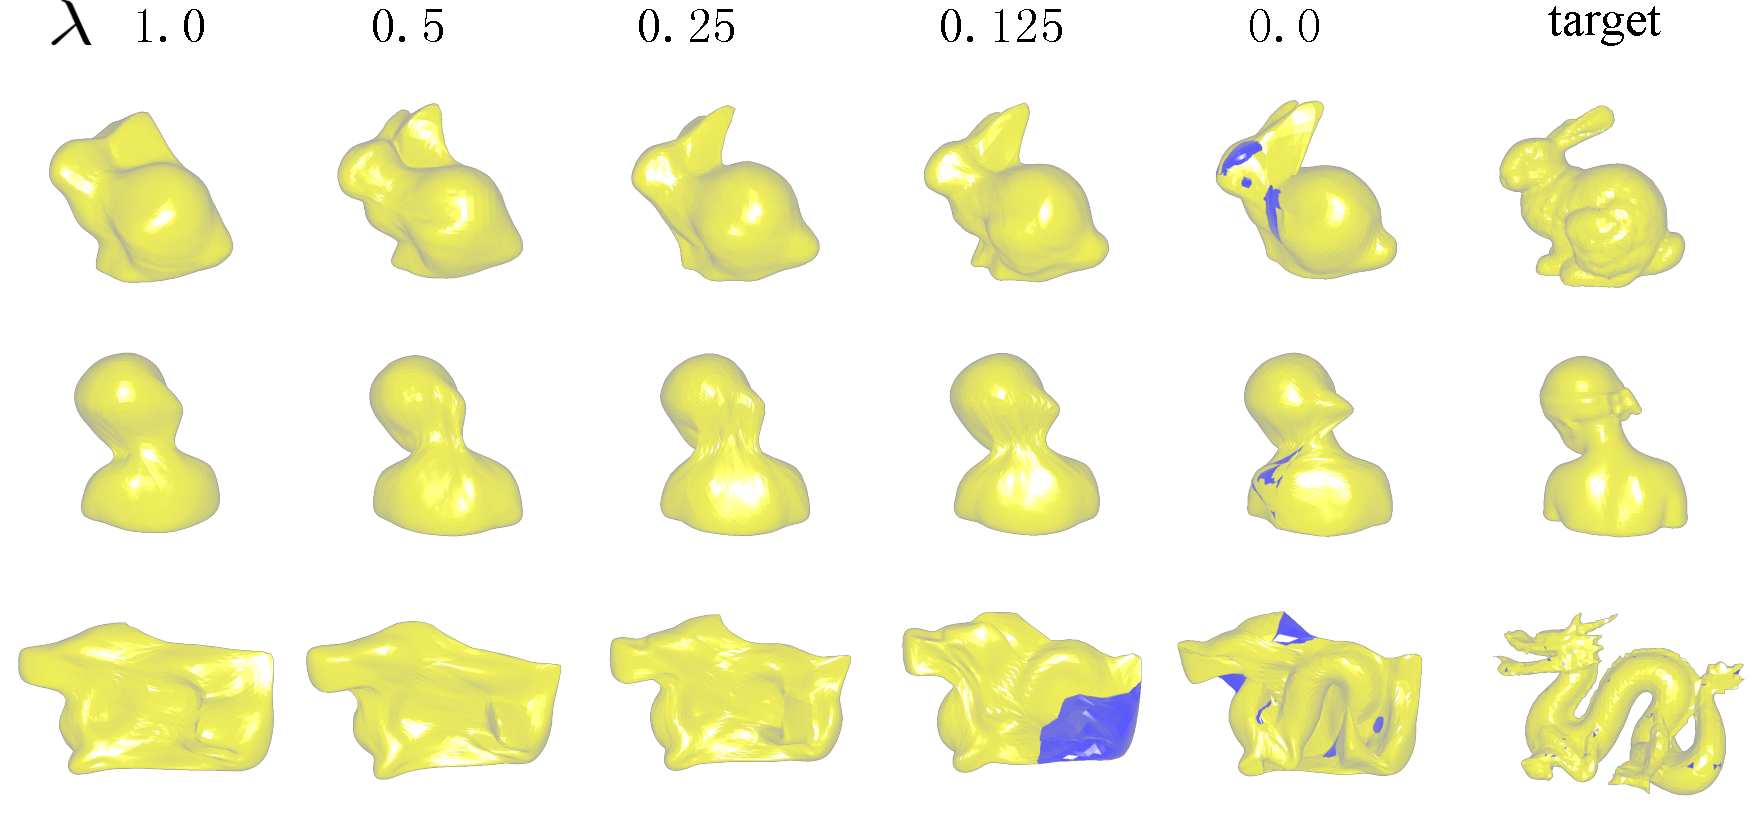
\includegraphics[width=0.48\textwidth]{img/opt/lambda}
	\end{center}
	\caption{The choice of $\lambda$: Under the setting in Sec~\ref{subsec:deform}, we show some results with different choice of $\lambda$}
	\label{fig:lambda}
\end{wrapfigure}

As shown in Figure~\ref{fig:lambda}, visually speaking, when we set the weight $\lambda=0.25$, the deformed shape is able to approximate more details than the larger choices (i.e. $\lambda=0.5,1.0$), and it is also sufficient to enforce the injective mapping.  Therefore we use $\lambda=0.25$ as an empirical choice in following experiments, however finer tuning for specific networks is possible. 
\subsection{Cycle regularization with AtlasNet}
In this subsection, we show and discuss the effect of our cycle regularization term on AtlasNet \cite{atlasnet}. As shown in Table~\ref{tab:atlas}, after applying our cycle regularization on the AtlasNet(sphere), the percentage of self-intersected triangles (``SI") are significantly reduced, while the Chamfer distance (``CD") remains close to original networks (somehow slightly worse in auto-encoding and better in single view reconstruction task). As visualized in Figure~\ref{fig:svr} for single view reconstruction task, the reduction of self-intersection is also visually evident. In some cases, as the one highlighted by red rectangles in Figure~\ref{fig:svr}, our cycle regularization term even helps to improve the reconstructed details.
\subsection{Cycle regularization with Pixel2Mesh}

\begin{table}
	\caption{Test error on Pixel2Mesh trained with(\textbf{ours}) and without cycle regularization. Chamfer distance(CD) and percentage of self-intersected(SI) faces are reported. The mean is data-wise calculated}
	\label{tab:p2m}
	\centering
	\begin{tabular}{c|rc|rc|}
		\diagbox{Category}{CD,SI}{Model}& \multicolumn{2}{c|}{without-cycle} & \multicolumn{2}{c|}{ours}\\
		\hline
		cellphone&0.303,&0.22\%&0.303,&3.85e-3\%\\
		watercraft&0.433,&0.84\%&0.438,&2.51e-2\%\\
		monitor&0.390,&0.585\%&0.425,&1.15e-2\%\\
		car&0.233,&0.145\%&0.242,&1.39e-3\%\\
		couch&0.361,&0.21\%&0.384,&3.67e-3\%\\
		cabinet&0.268,&0.167\%&0.283,&2.32e-3\%\\
		lamp&0.728,&10.3\%&0.788,&0.190\%\\
		plane&0.265,&1.82\%&0.300,&3.75e-2\%\\
		speaker&0.523,&0.487\%&0.524,&5.09e-3\%\\
		bench&0.323,&1.13\%&0.349,&3.32e-2\%\\
		table&0.304,&1.17\%&0.333,&4.98e-2\%\\
		chair&0.392,&1.68\%&0.420,&6.82e-2\%\\
		firearm&0.326,&1.86\%&0.352,&8.64e-2\%\\
		\hline
		mean &0.345,&1.47\%&0.369,& 1.3e-2\%\\
	\end{tabular}
\end{table}

\subsection{Limitations and future work}

When we apply our cycle regularization term to the model based on 25-patches, which is also released by AtlasNet \cite{atlasnet}, we encountered failure(for more details please turn to our supplemental material). We believe this is due to the reason we stated under \emph{Remaining gap} in Sec~\ref{subsec:cyclereg}. In fact, the AtlasNet based on 25-patches use 25 independent point-wise MLP to map the domain $[0,1]^2$ to different part of the target surface. This makes the overall mapping neither a canonical function (map one point from the patch to multiple points on surface) nor continue. In future, we want to try to use masks on continue domain instead of multiple patches to handle the cases in which the target surface is not homeomorphic to continue surface. This is how the researchers usually handle it for human mouth on the face surface in parameterization. We imagine it as using point-wise attention mechanism in mesh generation networks.